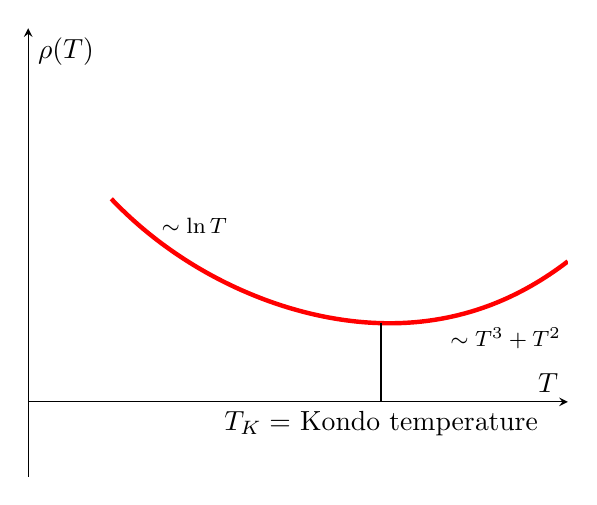
\begin{tikzpicture}
    \begin{axis}[
        xmin = 0.4, xmax = 1.7,
        ymin = -0.2, ymax = 1,
        axis lines = center,
        axis on top =true,
        domain = 0.6:1.7,
        restrict y to domain=0:1,
        ylabel = $\rho(T)$,
        xlabel = $T$,
        samples = 100,
        ticks = none
        ]
        
        \addplot[mark = none, draw = red, ultra thick]{0.07 * (6*ln(1/(x-0.25)) + (x-0.5)^2 +  1/3 * x^5) + 0.1};
        
        
    	\draw [thick] (axis cs:1.25,0)-- (axis cs:1.25,0.21);
    
        \node at (axis cs:0.8,0.47) {\footnotesize $\sim\ln T$};
        \node at (axis cs:1.55,0.17) {\footnotesize $\sim T^3 + T^2$};
       	\node[anchor = north] at (axis cs:1.25, 0) {$T_K = $ Kondo temperature};
        %\draw[->] (axis cs:3, 0.35) --(axis cs:4, 0.35) ;
    \end{axis}
\end{tikzpicture}